%! TeX program = pdflatex
\documentclass[pdflatex,sn-mathphys-num]{sn-jnl}
\usepackage{pgfplots}
\usepackage{amsmath}
\usepackage{algorithm}
\usepackage{algpseudocode}
\usepackage{subcaption}
\usepackage{float}
\pgfplotsset{compat=1.18}

\title[Automatic Multilevel Threshold]{%
  Automatic multilevel threshold using open-polygon search with mean and bin distance as stop condition
}
\author[1]{%
  \fnm{Brandon} \sur{Marquez-Salazar}
}
\email{b.marquezsalazar@ugto.mx}

\affil[1]{%
  \orgname{Universidad de Guanajuato}, \city{Guanajuato}, \country{Mexico}
}

\begin{document}
  \maketitle

  \begin{abstract}
    Thresholding is a specific case of contrast stretching where 
    the image intensities are clipped into binary values in terms of
    the image histogram \cite{Jain1988-ak}.
    By extension, the multilevel thresholding is a specific case of
    contrast stretching where the image is divided into several
    regions which are then thresholded separately, this processing
    helps in image analysis enhancing region segmentation and
    object detection.
  \end{abstract}

  \keywords{Image processing, Thresholding, Segmentation, Maxima search method}

  \section{Introduction}
  Thresholding is a common technique for segmentation in images, which is useful
  in different contexts where it is intended any object detection, contour detection,
  object detection, etc.
  Here, the main proposal is to generate a program which can automatically detect
  the maxima of an image histogram and then processing with a multilevel threshold.
  For this approach, it will be used an open-polygon search method which will be explained
  in the next section.

  \section{Methods}
  In this section, it will be explained the different processes needed to achieve 
  the proposed method.

  \subsection{Histogram}
  First of all, it is good to construct the histogram of the image which is made by:
  \begin{equation}
    H = \left[\sum_{j=0}^{n-1} \sum_{i=0}^{m-1} \phi_l(A_{ij})\right]_{l=0}^{255}
  \end{equation}
  where
  \begin{equation}
    \phi_l(A_{ij}) =
    \begin{cases}
      1 & \text{ if } l = A_{ij} \\
      0 & \text{ if } l \neq A_{ij}
    \end{cases}
  \end{equation}
  
  \subsection{Maxima search}
  For any multilevel thresholding is needed to specify the levels of reference, 
  so in this section it'll be explained the open-polygon search method.

  \begin{algorithm}
    \caption{Complete Histogram Maxima Detection}
    \begin{algorithmic}[1]
    \Require Histogram $H[0..L-1]$, Window size $s$
    \Ensure Binary maxima array $M[0..L-1]$, Count $N_{\text{maxima}}$
    \State Initialize $M[i] \gets \text{false}$ for $i = 0$ to $L-1$
    \State $N_{\text{maxima}} \gets 0$, $i \gets 0$
    \While{$i < L$}
        \State $w \gets \min(s, L - i)$
        \State $(found, pos) \gets \text{ConstrainedMaxima}(H, i, w)$
        \If{$found$}
            \State $M[i + pos] \gets \text{true}$
            \State $N_{\text{maxima}} \gets N_{\text{maxima}} + 1$
            \State $i \gets i + w$ \Comment{Skip processed polygon}
        \Else
            \State $i \gets i + 1$ \Comment{Continue search}
        \EndIf
    \EndWhile
    \State \Return $M, N_{\text{maxima}}$
    \end{algorithmic}
    \label{alg:complete_maxima}
    \end{algorithm}

    \begin{algorithmic}[1]
    \Function{ConstrainedMaxima}{$H$, $start$, $width$}
        \If{$width = 0$} \Return $(\text{false}, 0)$ \EndIf
        \State $\mu \gets \frac{1}{width} \sum_{j=0}^{width-1} H[start + j]$ \Comment{Polygon mean}
        \State $\delta \gets width / 2$ \Comment{Position constraint}
        \State $maxid \gets 0$
        \For{$j \gets 1$ to $width-1$}
            \If{$H[start + j] > H[start + maxid]$}
                \State $maxid \gets j$
            \EndIf
        \EndFor
        \State $found \gets (H[start + maxid] > \mu) \land (maxid < \delta)$
        \State \Return $(found, maxid)$
    \EndFunction
    \end{algorithmic}

  The search for the test images were made with a width of 80


  \section{Results}
  The results obtained where a full automatic multilevel thresholding.

% ===== TEST IMAGE 1 =====
\begin{figure}[H]
  \centering
  % Test 1: Original image
  \begin{subfigure}[b]{0.45\textwidth}
    \centering
    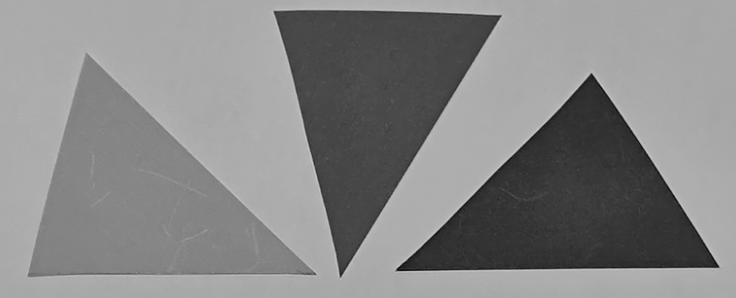
\includegraphics[width=0.9\textwidth]{./img.png/HistoTest01.png}
    \caption{Test 1: Original}
    \label{fig:test1-orig}
  \end{subfigure}
  \hfill
  % Test 1: Original Histogram
  \begin{subfigure}[b]{0.45\textwidth}
    \centering
    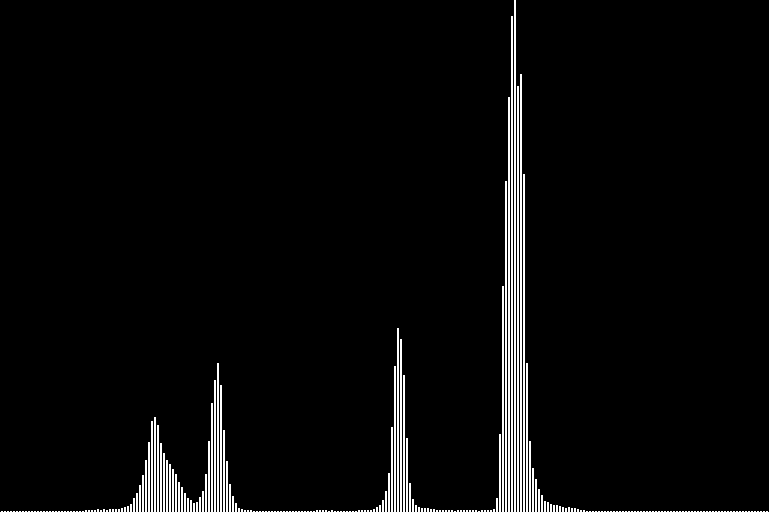
\includegraphics[width=0.9\textwidth]{./img.png/Histogram_of_HistoTest01.png}
    \caption{Test 1: Original Histogram}
    \label{fig:test1-hist-orig}
  \end{subfigure}
  
  % Test 1: Thresholded
  \begin{subfigure}[b]{0.45\textwidth}
    \centering
    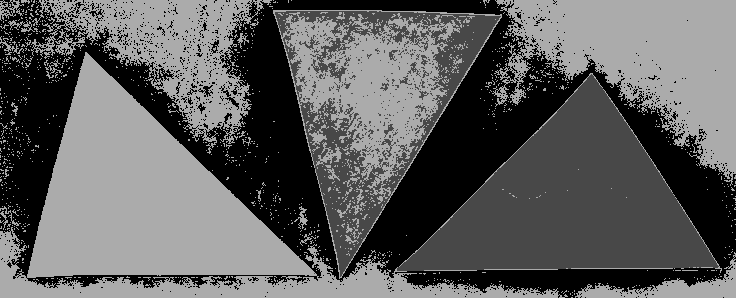
\includegraphics[width=0.9\textwidth]{./img.png/HistoTest01_Thres.png}
    \caption{Test 1: Thresholded}
    \label{fig:test1-thres}
  \end{subfigure}
  \hfill
  % Test 1: Thresholded Histogram
  \begin{subfigure}[b]{0.45\textwidth}
    \centering
    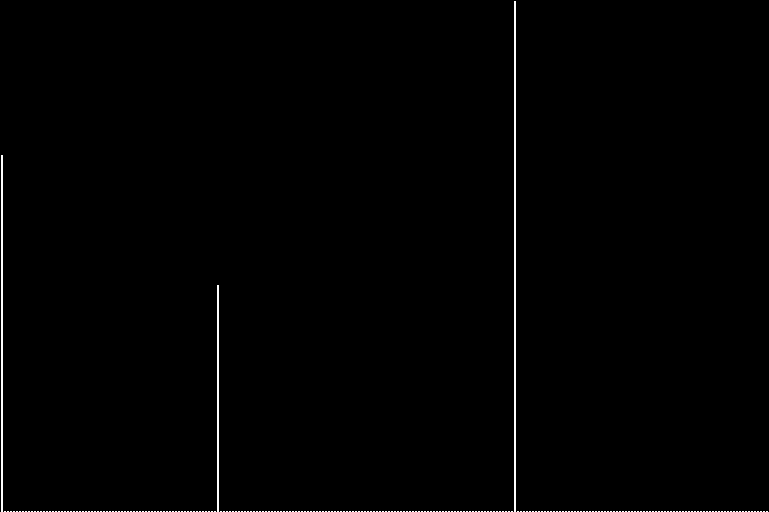
\includegraphics[width=0.9\textwidth]{./img.png/Histogram_of_HistoTest01_Thres.png}
    \caption{Test 1: Thresholded Histogram}
    \label{fig:test1-hist-thres}
  \end{subfigure}
  
  \caption{Comparative analysis of thresholding results for HistoTest01.bmp}
  \label{fig:comparative-test1}
\end{figure}

% ===== TEST IMAGE 2 =====
\begin{figure}[H]
  \centering
  % Test 2: Original image
  \begin{subfigure}[b]{0.45\textwidth}
    \centering
    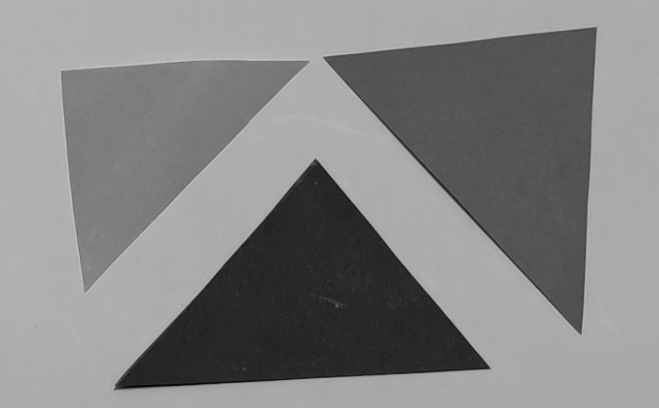
\includegraphics[width=0.9\textwidth]{./img.png/HistoTest02.png}
    \caption{Test 2: Original}
    \label{fig:test2-orig}
  \end{subfigure}
  \hfill
  % Test 2: Original Histogram
  \begin{subfigure}[b]{0.45\textwidth}
    \centering
    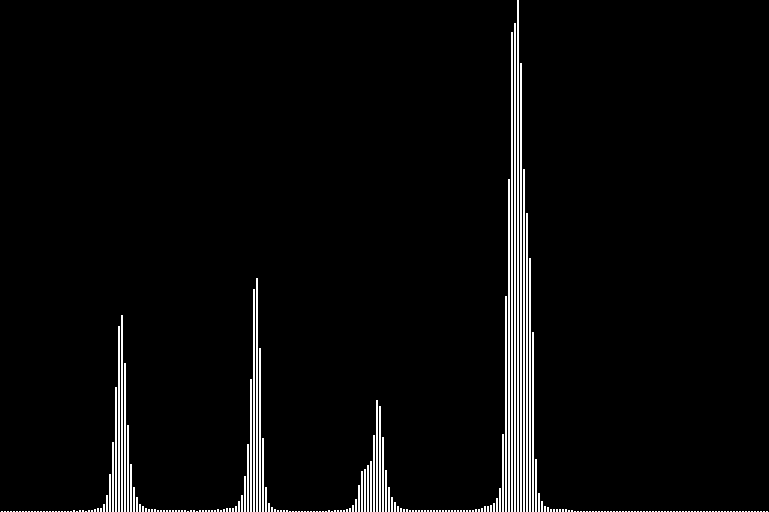
\includegraphics[width=0.9\textwidth]{./img.png/Histogram_of_HistoTest02.png}
    \caption{Test 2: Original Histogram}
    \label{fig:test2-hist-orig}
  \end{subfigure}
  
  % Test 2: Thresholded
  \begin{subfigure}[b]{0.45\textwidth}
    \centering
    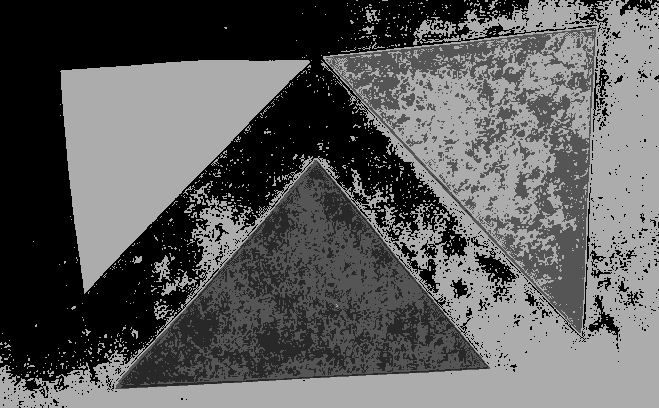
\includegraphics[width=0.9\textwidth]{./img.png/HistoTest02_Thres.png}
    \caption{Test 2: Thresholded}
    \label{fig:test2-thres}
  \end{subfigure}
  \hfill
  % Test 2: Thresholded Histogram
  \begin{subfigure}[b]{0.45\textwidth}
    \centering
    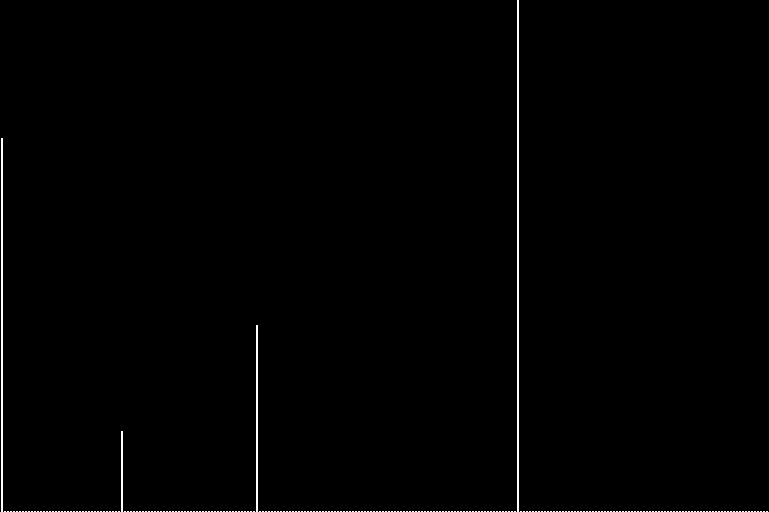
\includegraphics[width=0.9\textwidth]{./img.png/Histogram_of_HistoTest02_Thres.png}
    \caption{Test 2: Thresholded Histogram}
    \label{fig:test2-hist-thres}
  \end{subfigure}
  
  \caption{Comparative analysis of thresholding results for HistoTest02.bmp}
  \label{fig:comparative-test2}
\end{figure}

% ===== TEST IMAGE 3 =====
\begin{figure}[H]
  \centering
  % Test 3: Original image
  \begin{subfigure}[b]{0.45\textwidth}
    \centering
    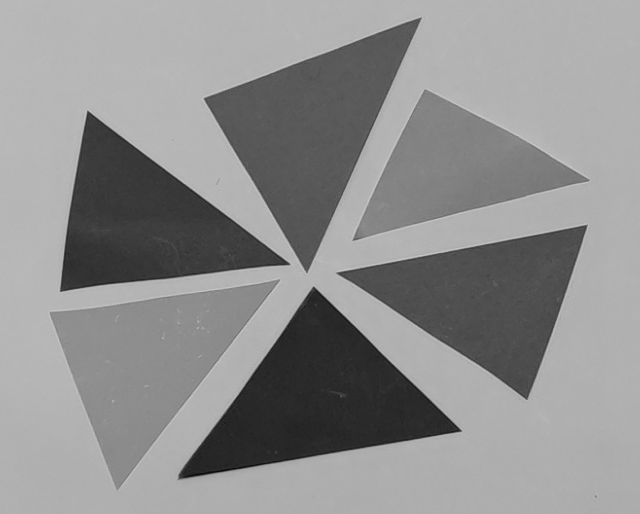
\includegraphics[width=0.9\textwidth]{./img.png/HistoTest03.png}
    \caption{Test 3: Original}
    \label{fig:test3-orig}
  \end{subfigure}
  \hfill
  % Test 3: Original Histogram
  \begin{subfigure}[b]{0.45\textwidth}
    \centering
    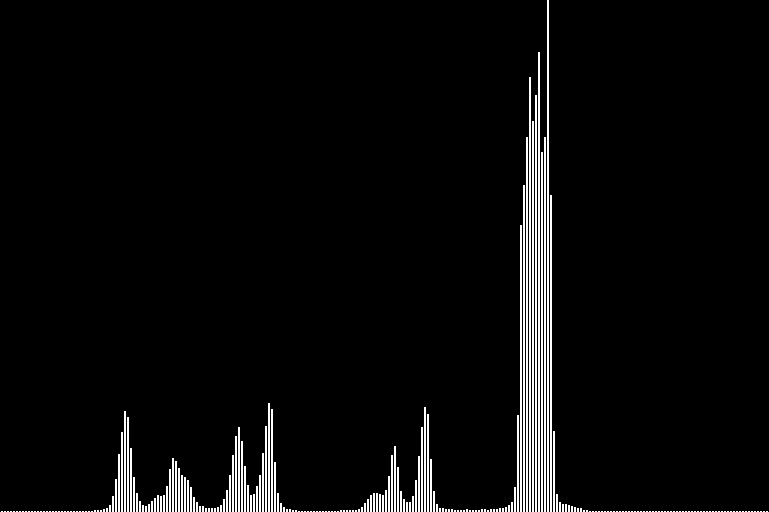
\includegraphics[width=0.9\textwidth]{./img.png/Histogram_of_HistoTest03.png}
    \caption{Test 3: Original Histogram}
    \label{fig:test3-hist-orig}
  \end{subfigure}
  
  % Test 3: Thresholded
  \begin{subfigure}[b]{0.45\textwidth}
    \centering
    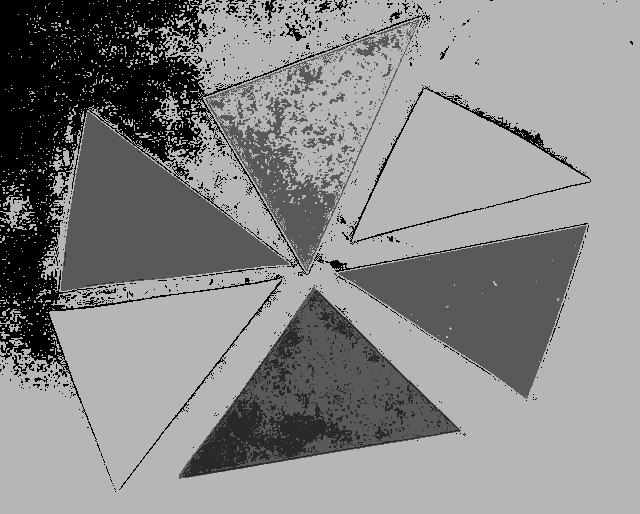
\includegraphics[width=0.9\textwidth]{./img.png/HistoTest03_Thres.png}
    \caption{Test 3: Thresholded}
    \label{fig:test3-thres}
  \end{subfigure}
  \hfill
  % Test 3: Thresholded Histogram
  \begin{subfigure}[b]{0.45\textwidth}
    \centering
    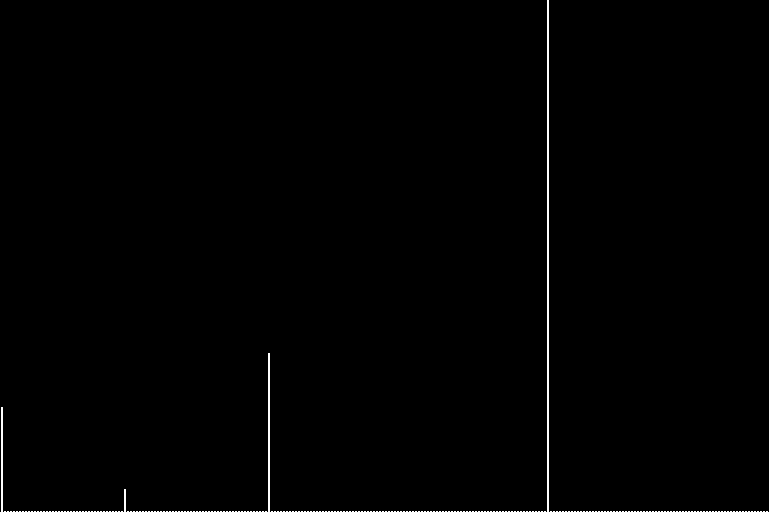
\includegraphics[width=0.9\textwidth]{./img.png/Histogram_of_HistoTest03_Thres.png}
    \caption{Test 3: Thresholded Histogram}
    \label{fig:test3-hist-thres}
  \end{subfigure}
  
  \caption{Comparative analysis of thresholding results for HistoTest03.bmp}
  \label{fig:comparative-test3}
\end{figure}

% ===== REAL TEST IMAGE 1 =====
\begin{figure}[H]
  \centering
  % Real Test 1: Original image
  \begin{subfigure}[b]{0.45\textwidth}
    \centering
    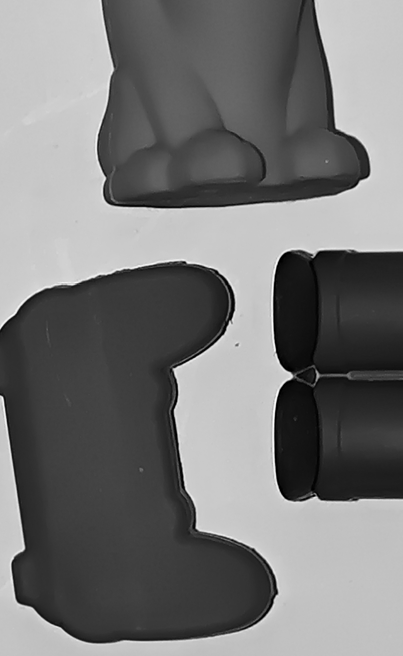
\includegraphics[width=0.9\textwidth]{./img.png/HistoTestReal01.png}
    \caption{Real Test 1: Original}
    \label{fig:realtest1-orig}
  \end{subfigure}
  \hfill
  % Real Test 1: Original Histogram
  \begin{subfigure}[b]{0.45\textwidth}
    \centering
    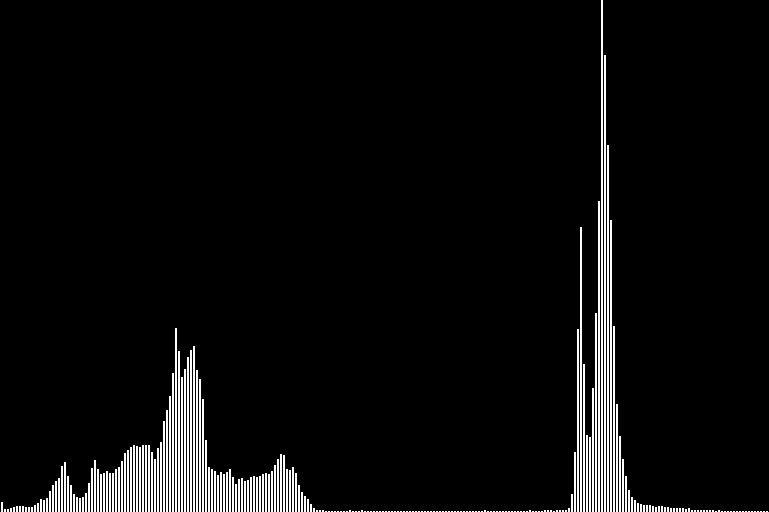
\includegraphics[width=0.9\textwidth]{./img.png/Histogram_of_HistoTestReal01.png}
    \caption{Real Test 1: Original Histogram}
    \label{fig:realtest1-hist-orig}
  \end{subfigure}
  
  % Real Test 1: Thresholded
  \begin{subfigure}[b]{0.45\textwidth}
    \centering
    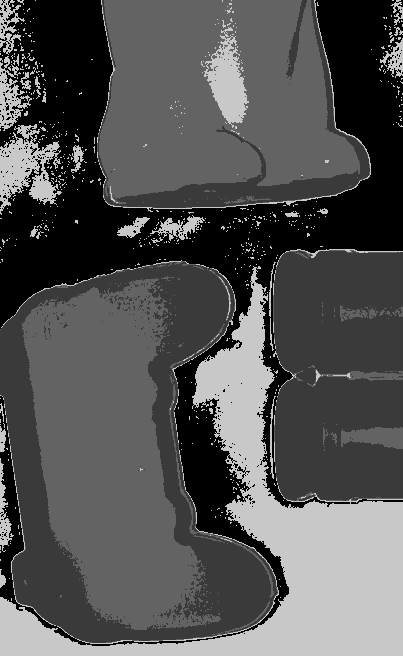
\includegraphics[width=0.9\textwidth]{./img.png/HistoTestReal01_Thres.png}
    \caption{Real Test 1: Thresholded}
    \label{fig:realtest1-thres}
  \end{subfigure}
  \hfill
  % Real Test 1: Thresholded Histogram
  \begin{subfigure}[b]{0.45\textwidth}
    \centering
    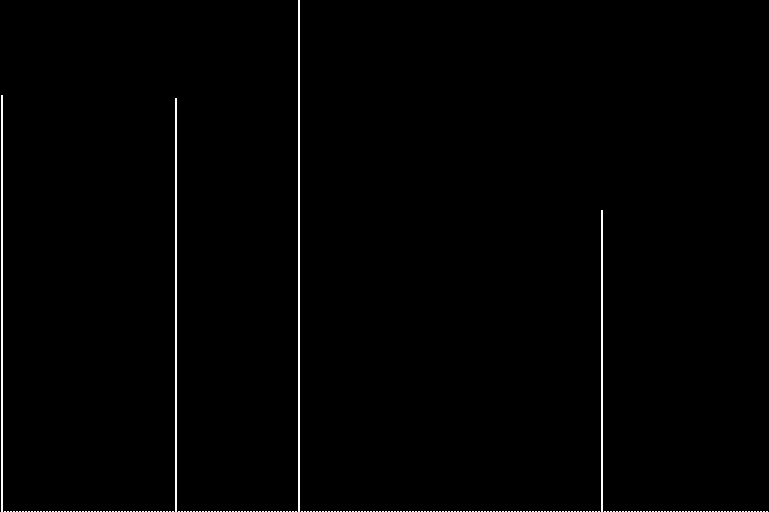
\includegraphics[width=0.9\textwidth]{./img.png/Histogram_of_HistoTestReal01_Thres.png}
    \caption{Real Test 1: Thresholded Histogram}
    \label{fig:realtest1-hist-thres}
  \end{subfigure}
  
  \caption{Comparative analysis of thresholding results for HistoTestReal01.bmp}
  \label{fig:comparative-realtest1}
\end{figure}

% ===== REAL TEST IMAGE 2 =====
\begin{figure}[H]
  \centering
  % Real Test 2: Original image
  \begin{subfigure}[b]{0.45\textwidth}
    \centering
    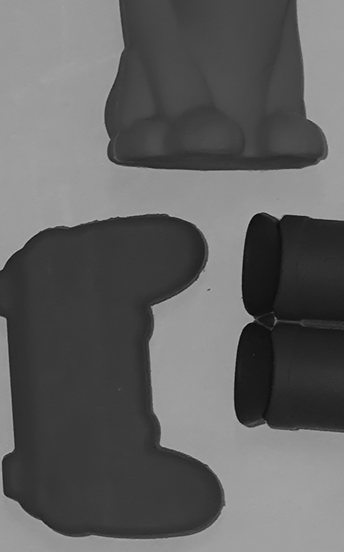
\includegraphics[width=0.9\textwidth]{./img.png/HistoTestReal02.png}
    \caption{Real Test 2: Original}
    \label{fig:realtest2-orig}
  \end{subfigure}
  \hfill
  % Real Test 2: Original Histogram
  \begin{subfigure}[b]{0.45\textwidth}
    \centering
    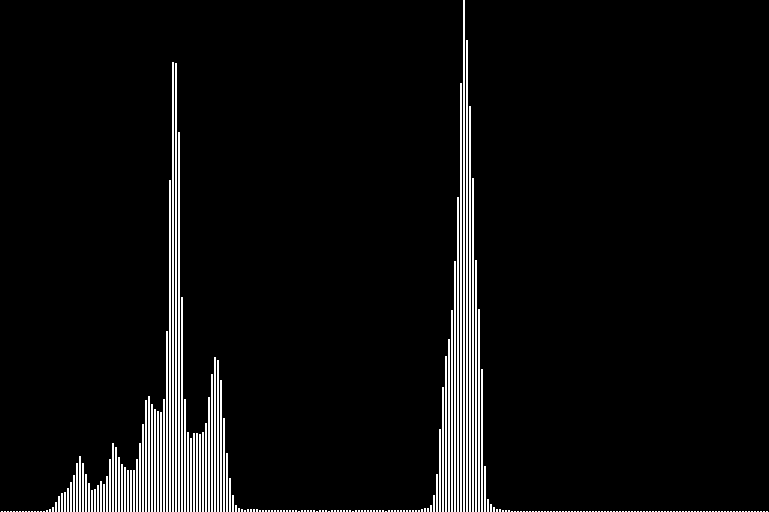
\includegraphics[width=0.9\textwidth]{./img.png/Histogram_of_HistoTestReal02.png}
    \caption{Real Test 2: Original Histogram}
    \label{fig:realtest2-hist-orig}
  \end{subfigure}
  
  % Real Test 2: Thresholded
  \begin{subfigure}[b]{0.45\textwidth}
    \centering
    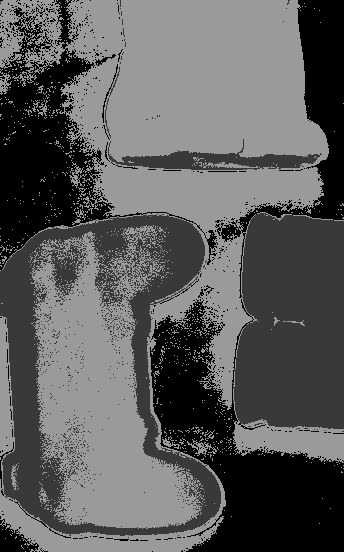
\includegraphics[width=0.9\textwidth]{./img.png/HistoTestReal02_Thres.png}
    \caption{Real Test 2: Thresholded}
    \label{fig:realtest2-thres}
  \end{subfigure}
  \hfill
  % Real Test 2: Thresholded Histogram
  \begin{subfigure}[b]{0.45\textwidth}
    \centering
    
\includegraphics[width=0.9\textwidth]{./img.png/Histogram_of_HistoTestReal02_Thres.png}
    \caption{Real Test 2: Thresholded Histogram}
    \label{fig:realtest2-hist-thres}
  \end{subfigure}
  
  \caption{Comparative analysis of thresholding results for HistoTestReal02.bmp}
  \label{fig:comparative-realtest2}
\end{figure}

% ===== REAL TEST IMAGE 3 =====
\begin{figure}[H]
  \centering
  % Real Test 3: Original image
  \begin{subfigure}[b]{0.45\textwidth}
    \centering
    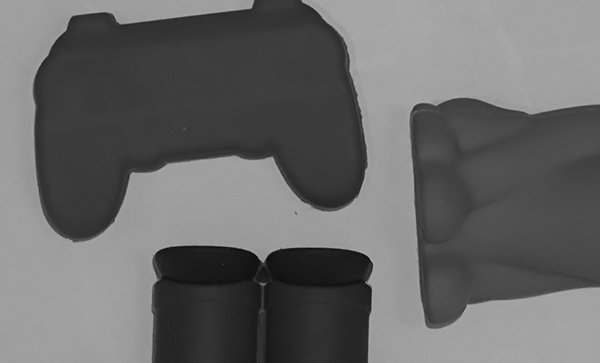
\includegraphics[width=0.9\textwidth]{./img.png/HistoTestReal03.png}
    \caption{Real Test 3: Original}
    \label{fig:realtest3-orig}
  \end{subfigure}
  \hfill
  % Real Test 3: Original Histogram
  \begin{subfigure}[b]{0.45\textwidth}
    \centering
    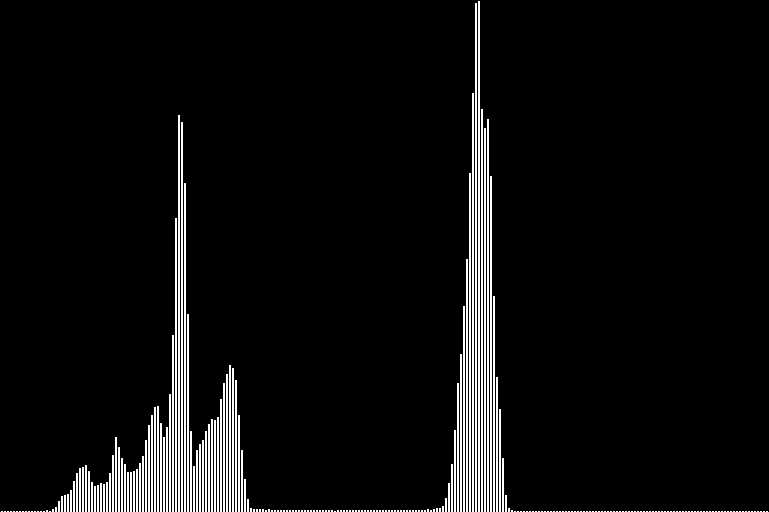
\includegraphics[width=0.9\textwidth]{./img.png/Histogram_of_HistoTestReal03.png}
    \caption{Real Test 3: Original Histogram}
    \label{fig:realtest3-hist-orig}
  \end{subfigure}
  
  % Real Test 3: Thresholded
  \begin{subfigure}[b]{0.45\textwidth}
    \centering
    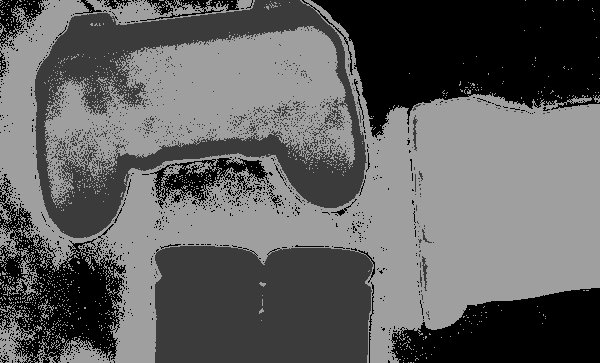
\includegraphics[width=0.9\textwidth]{./img.png/HistoTestReal03_Thres.png}
    \caption{Real Test 3: Thresholded}
    \label{fig:realtest3-thres}
  \end{subfigure}
  \hfill
  % Real Test 3: Thresholded Histogram
  \begin{subfigure}[b]{0.45\textwidth}
    \centering
    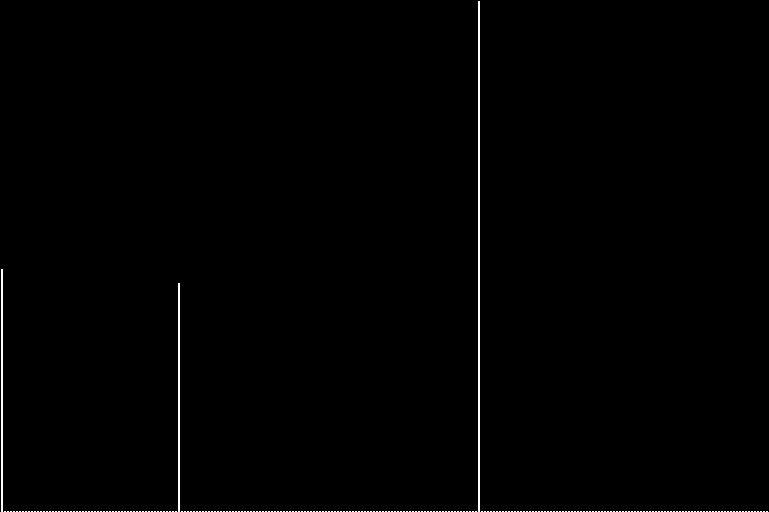
\includegraphics[width=0.9\textwidth]{./img.png/Histogram_of_HistoTestReal03_Thres.png}
    \caption{Real Test 3: Thresholded Histogram}
    \label{fig:realtest3-hist-thres}
  \end{subfigure}
  
  \caption{Comparative analysis of thresholding results for HistoTestReal03.bmp}
  \label{fig:comparative-realtest3}
\end{figure}
  
\newpage

  \section{Discussion}
  The code is fully functional which can be useful in different contexts, however, there is as in every tool cases where it can perform better than others.
  The main point is to search a bin distance which can be optimum for each image and light conditions.

  \section{Conclusion}
  In this work it was proposed a method to automatically detect the maxima of an image histogram and then processing with a multilevel threshold
  which can be useful in different contexts where it is intended any object detection, contour detection, object detection, etc.

  The main goal was achieved, but regarding that the bin distance for this approach should be tuned depending on the image needs and features.

  It can be later used in HSV space for color segmentation, and it should be useful for binarizaton by putting a width of 256.

  This approach is also perfectible, so this is the first step in this project.

  \bibliography{bib}
\end{document}
